\documentclass[a4paper,twocolumn,10pt]{article}
\usepackage[spanish]{babel}
\usepackage[T1]{fontenc}
\usepackage[utf8]{inputenc}
\spanishdecimal{.}
\usepackage{lmodern}
\usepackage[a4paper]{geometry}
\usepackage{graphicx}
\usepackage{flushend}
\usepackage{wallpaper}
\usepackage{float}
\usepackage{colortbl}

\begin{document}

\title{Determinación de la relación carga-masa para el electrón}
\author{ \\Aldo Aliaga, Benjamín Yapur, Fabian Trigo \\ \textit{Departamento de Física y Astronomía, Universidad de Valparaiso}}
\twocolumn[
  \begin{@twocolumnfalse}
    \maketitle
    \begin{abstract}
        Este experimento tiene como objetivo la determinación de la fracción carga por masa del electrón, se utiliza una cavidad al vació donde se aceleran los electrones y mediante bobinas se dirige en una circunferencia. Obteniendo la medida con su incertidumbre: $\frac{q}{m} = (2.81 \pm 1.46) \times 10^{11} C/Kg$ , difiriendo del valor de la literatura por un $59\%$, predicha por la incertidumbre sistematica de $83\%$.
      
    \end{abstract}
  \end{@twocolumnfalse}
]
  
\section{Introducción}
De la fuerza de Lorentz, tenemos como los campos electrostáticos y magnéticos afectan a las cargas:
$$
\vec F = q\vec E + q \vec v \times \vec B
$$
\subsection{Electrostática}
La fuerza electrostática acelera a la carga, aumentando su velocidad:
$$
F_{elec} = q E
$$
ha de considerarse la cantidad de energía que provoca tener un campo eléctrico,
$$
W = -q\int \vec E \cdot d \vec l = q \Delta V
$$
la energía que adquiere una carga es proporcional al voltaje por su carga, de ahí que toda se convierta en energía cinética clásica:
$$
\frac{1}{2}m v^2 = q V
$$
se ve entonces la cantidad deseada $q/m$:
\begin{equation}
    v^2 = 2V \frac{q}{m}
\end{equation}\label{cinetica}



\subsection{Magnetoestatica}
De la fuerza de Lorentz, extraer la fuerza magnética que afecta a las cargas en movimiento,
$$ F_{mag}= q \vec{v} \times \vec{B} $$
para una carga en linea recta, la acelera de manera perpendicular a su velocidad, de manera que provoca una circunferencia; para una circunferencia la fuerza centrípeta a de ser proporcional a la velocidad al cuadrado $v^2$ dividida por el radio $R$:
$$
|F_{cent}| = m \frac{v^2}{R}
$$
Igualando la fuerza magnética a la centrípeta, $|F_{mag}| = |F_{cent}|$:
$$
q v B = m \frac{v^2}{R}
$$
despejando para la cantidad deseada,
\begin{equation}
    v = \frac{q}{m} \frac{R}{B}
\end{equation}\label{centripeta}

\subsection{Despejar factor carga sobre masa}
Entonces combinando las ecuaciones \ref{cinetica} y \ref{centripeta}:
$$
\begin{array}{cc}
    v^2 = v^2  \\
      (\frac{q}{m} \frac{R}{B})^2 =  2V \frac{q}{m} \\
      \frac{q}{m} = \frac{2V}{B^2 R^2}
\end{array}
$$

De esa manera la ecuacion que guia este fenomeno
\begin{equation}
    \frac{q}{m} = \frac{2V}{(RB)^2}
\end{equation}\label{maineq}


\section{Montaje Experimental}
\subsection{Herramientas}
\begin{itemize} 
\item Bobinas de Helmholtz
\item Tester 
\item Tubo de haz fino sobre zócalo de conexión R
\item Fuente de alimentación de CC 0 – 500 V (230mani V, 50/60 Hz)
\end{itemize}

\subsection{Procedimiento experimental}

En primer lugar se tienen las bobinas de Helmholtz que crean un campo magnético al circular una corriente a través de sus espiras. Entre ambas bobinas se localiza la bombilla en la que circulan los electrones. 

Por otro lado se tiene la fuente de alimentación, la cual proporciona los voltajes y corrientes necesarias para la instrumentación ubicada en las bobinas.

Además se utilizan dos multitester, uno en modo voltímetro para conocer el voltaje con que se aceleran los electrones y otro en modo amperímetro para precisar la corriente que pasa por las bobinas.

La fuente de alimentación consta de 4 controles (Ver Figura 1), se detallan a continuación de izquierda a derecha:

El primer control establece la diferencia de potencial que acelera los electrones, se varía el voltaje varias veces para cada valor de corriente.

El segundo control es el encargado de colimar el haz de electrones. Esta se deja fijo de modo que el haz sea fácil de resolver y no esté muy disperso para no tener complicaciones al momento de medir el radio de la trayectoria.

El tercer control se conecta a un multitester en modo amperímetro para así controlar la corriente que fluye por las bobinas. Luego, el tester se conecta a uno de los casquillos de las bobinas para que la corriente circule por ellas, la corriente pasa por toda esta bobina y es transmitida hacía la bobina que se encuentra en la parte anterior de la Figura 1. La corriente fluye por toda esta bobina y se conecta de vuelta a la batería para tener el circuito cerrado.

La corriente se modifica en función de controlar la trayectoria circular de los electrones. Alterando el campo magnético y así obtener una trayectoria con el radio que se quiera medir.

El cuarto control regula el flujo de electrones. Se mantiene fijo con un voltaje menor a $6[V]$ para evitar dañar el filamento de caldeo. Este último control es conectado a un tester en modo voltímetro para estar seguros de no sobrepasar dicho límite

\begin{figure}[H]
    \centering
    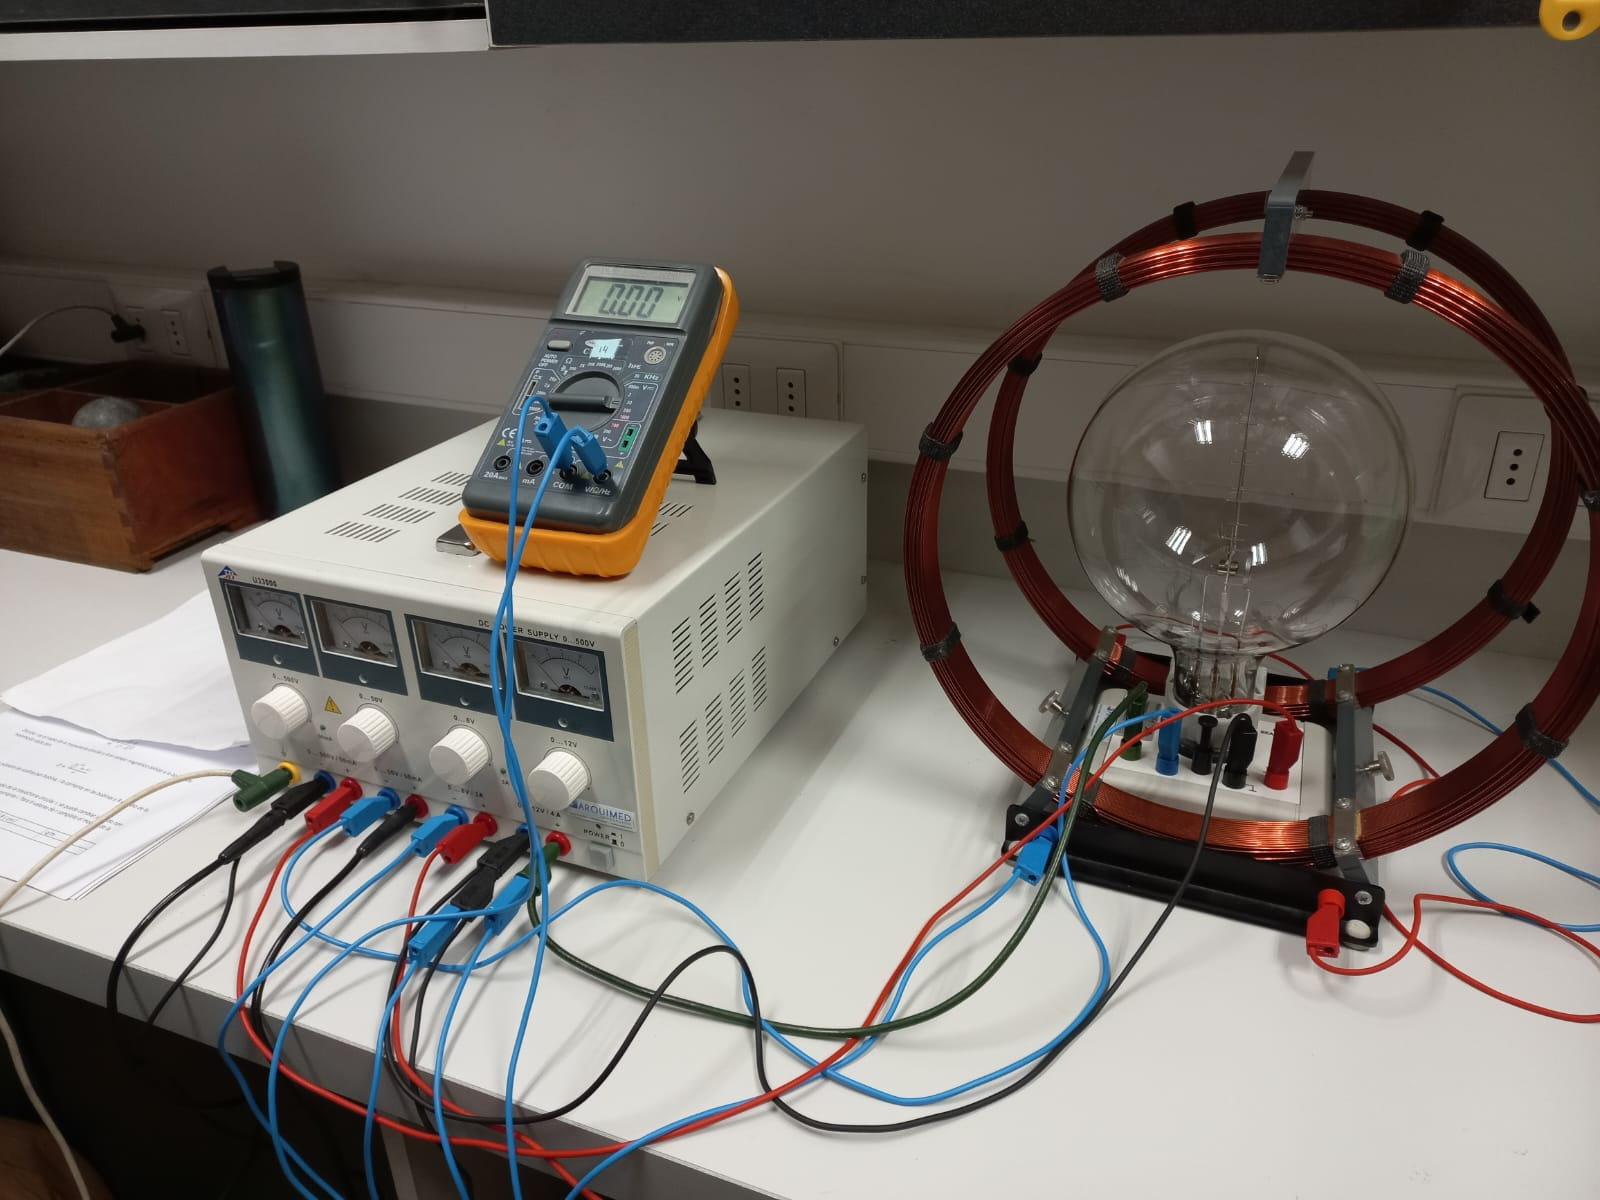
\includegraphics[width=0.45\textwidth]{montaje.jpeg}
    \caption{Montaje de experimento.}
    \label{fig:montaje_foto_real}
\end{figure}

Las conexiones:
\begin{figure}[H]
    \centering
    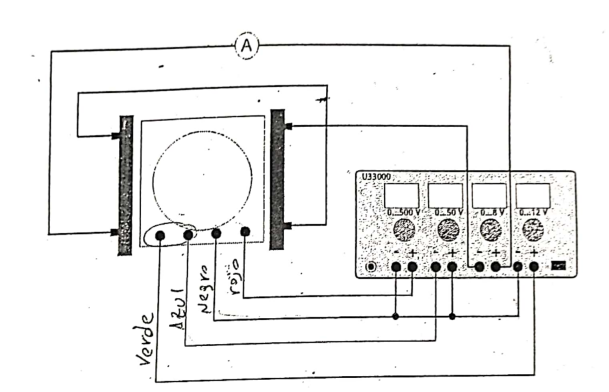
\includegraphics[width=0.45\textwidth]{Imagenes/QM/hazfinoafuente.png}
    \caption{Montaje de experimento.}
    \label{fig:montaje_hazfinofuente}
\end{figure}

\begin{figure}[H]
    \centering
    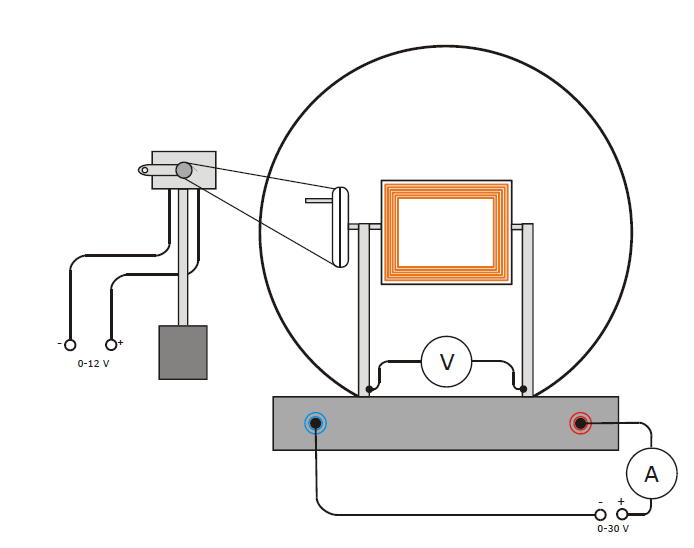
\includegraphics[width=0.45\textwidth]{Imagenes/QM/montajebola.png}
    \caption{Montaje de experimento.}
    \label{fig:montaje_bola}
\end{figure}




\section{Análisis}
\subsection{Limites de Precisión}
Los limites de precisión experimentales se define por sus constituyentes:
\begin{itemize}
    \item Las variables del experimento
    \item Las funciones, que controlan las variables
    \item Las ecuaciones que rigen a la física
    \item Las incertidumbres del equipo
\end{itemize}
como un algoritmo para obtener 

De acuerdo a las especificaciones de manufactura de las bobinas solídales, el campo magnetico producto de las dos bobinas es función de la Corriente:

$$ B(I) = 7.34  \times 10^{-4} \cdot I \:\:[T]$$

Entre el aire y el vacío la diferencia de la permeabilidad magnética es insignificativa comparada a otras incertidumbres (B. D. Cullity and C. D. Graham (2008)) $\mu/\mu_0 = 1.00000037$, por tanto no se hizo diferencia en el cálculo de cambiar de medio en el campo magnético, nótese que debería de entonces tenerse en cuenta la geometría exacta de la bola de cristal.

%% Calculando el error 
La incertidumbre de $\mu = q/m$ fue calculado con:
$$
(\Delta \mu)^2 = \sum_i (\frac{\partial \mu}{\partial x_i} \Delta x_i)^2
$$
Conociendo las incertidumbres de cada variable $x_i$ fue posible predecir la incertidumbre de la función como tal:

$$
(\Delta \mu)^2 = (\frac{1}{B^3} \frac{2V}{R^2} \Delta B)^2 + (\frac{2}{(BR)^2} \Delta V)^2 + (\frac{1}{R^3} \frac{2V}{B^2} \Delta B)^2
$$

Con las incertidumbre del campo de inducción magnética $\Delta B = 7.34 \times 10^{-6}$, la cual proviene de la incertidumbre de la corriente multiplicada por una constante (Véase la manera de calcular el campo Magnético al comienzo de la sección de análisis), entonces listadas todas juntas:
\begin{itemize}
\item $\Delta I = 1 \times 10^{-2} [A]$
\item $\Delta B = 7.34 \times 10^{-6} [T] $
\item $\Delta R = 5 \times 10^{-3} [m]$
\item $\Delta V = 20 [Volts]$
\end{itemize}

Conseguimos la incertidumbre máxima, maximizando las funciones con los campos y voltaje más intensos, mientras que el radio más pequeño medido, definiendo así el limite superior del error:

$$ \Delta \mu \leq 6.847 \times 10^{11} [C/kg]$$

Reemplazando por los valores centrales que separan los datos un $50\%$, llamados medianas, definimos el error mediano:

$$ \Delta \mu = 1.46 \times 10^{11} [C/kg]$$

Teniendo en cuenta las incertidumbres se procedió a medir Voltaje, Corriente y el Radio de la circunferencia dibujada por la carga usando las lineas equiespaciadas dentro de la esfera al vacío, véase tabla \ref{fig:qmboxplot}

Se calcula una lista de $\mu$, la cual es graficada en la siguiente figura:

%grafico de dispersión %
\begin{figure}[H]
    \centering
    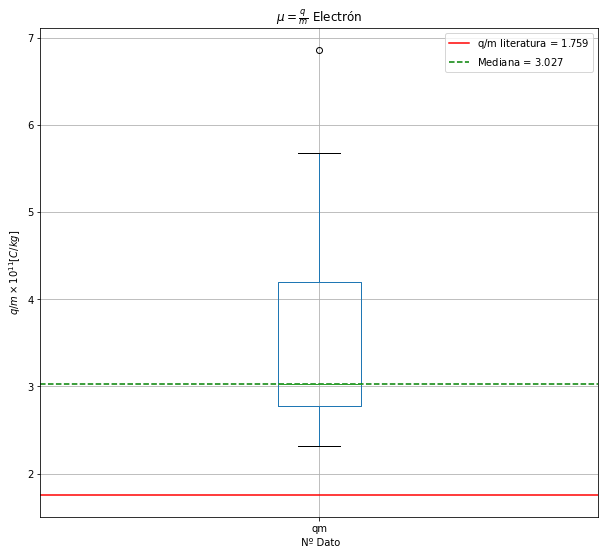
\includegraphics[width=0.5\textwidth]{PlotQM/Dispersionqm_1.png}
    \caption{Boxplot de la lista de $\mu$, donde la linea verde es la mediana de los datos, la linea roja es el valor proveniente de la literatura con el cual comparamos nuestros resultados para medir el error}
    \label{fig:qmboxplot}
\end{figure}

Dentro de la caja en el boxplot se encuentra el rango intercuartil, osea entre el $25\%$ y el $75\%$, teniendo allí el $50\%$ de los datos, luego los bigotes externos de la caja se extienden a 3 rangos intercuartiles o IQR o hasta encontrar el dato más lejano. Cuando se calculan los bigotes externos y quedan datos fuera a estos se les considera outliers o datos atípicos, este dato será ignorado, referente a: $\mu = 6.86 \times 10^{11} [C/kg]$

Luego de ignorar ese dato, se obtiene una nueva mediana aún más cercana al valor de literatura, como también se reduce con creces la dispersión, siendo ahora de una desviación estándar de $|\sigma| = 0.41 \times 10^{11}$; la tabla de datos ignorando este ultimo:


\begin{table}
\centering
\caption{Mediciones de Voltaje, Corriente y Radio observado, entonces provocando ciertos valores de q/m}
\begin{tabular}{rrrr}
\rowcolor[rgb]{0.753,0.753,0.753} \multicolumn{1}{l}{Volts} & \multicolumn{1}{l}{Corriente [A]} & \multicolumn{1}{l}{Radio [m]} & \multicolumn{1}{l}{$\frac{q}{m}$ $10^{11}$ [C/Kg] }  \\
140                                                         & -0.89                             & 0.050                         & 2.62                              \\
120                                                         & -1.00                             & 0.040                         & 2.78                              \\
110                                                         & -0.99                             & 0.035                         & 3.40                              \\
100                                                         & -0.99                             & 0.030                         & 4.20                              \\
90                                                          & -0.99                             & 0.025                         & 5.45                              \\
60                                                          & -0.99                             & 0.020                         & 5.68                              \\
290                                                         & -1.40                             & 0.045                         & 2.71                              \\
240                                                         & -1.40                             & 0.040                         & 2.84                              \\
180                                                         & -1.40                             & 0.035                         & 2.78                              \\
140                                                         & -1.40                             & 0.030                         & 2.94                              \\
100                                                         & -1.40                             & 0.025                         & 3.03                              \\
80                                                          & -1.42                             & 0.020                         & 3.68                              \\
80                                                          & -2.00                             & 0.015                         & 3.30                              \\
100                                                         & -2.00                             & 0.020                         & 2.32                              \\
180                                                         & -2.00                             & 0.025                         & 2.67                              \\
240                                                         & -1.98                             & 0.020                         & 5.68                             
\end{tabular}
\end{table}


%grafico de dispersión corregido %
\begin{figure}[H]
    \centering
    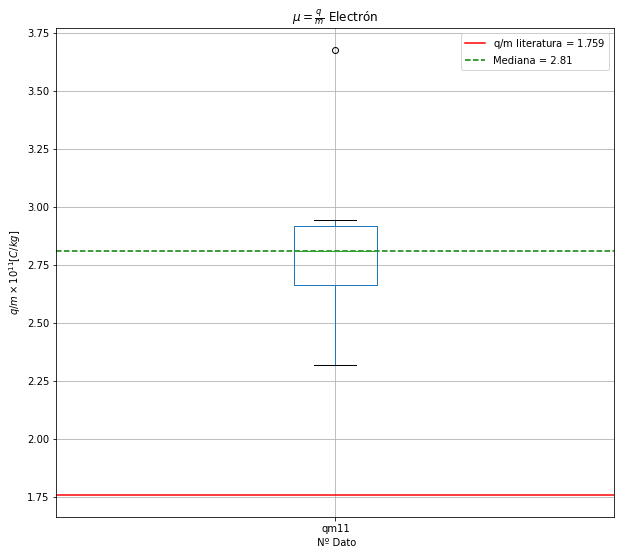
\includegraphics[width=0.5\textwidth]{PlotQM/dispersion_sin_outliers.png}
    \caption{2do Boxplot de la list de $\mu$, donde la linea verde es la mediana de los datos, la linea roja es el valor proviniente de la literatura con el cual comparamos nuestros resultados para medir el error}
    \label{fig:qmboxplot_noo}
\end{figure}

Se calcula el valor final de $mu$ como
$$
\mu = \frac{q}{m} = 2.81 \times 10^{11} [C/kg]
$$

El valor que se obtiene al calcular la carga del electrón y la masa conocidos actualmente:
$$
\frac{q}{m}_{real} = 1.76 \times 10^{11} [C/kg]
$$

Si reescribimos el error calculado previamente de manera porcentual, osea la incertidumbre porcentual:
$$
\epsilon_{\%} = \frac{ 1.46 \times 10^{11}}{1.76 \times 10^{11}} = 0.83
$$
osea que podemos esperar un error de un $83\%$, mediante un análisis de las fuentes de error usando Python, la esta gran contribución proviene de la incertidumbre al medir el radio de la circunferencia de iones.

Comparando el valor experimental al proveniente de la literatura al dividir la carga del electrón sobre su masa, obtenemos el error porcentual:
$$
\epsilon_{exp} = \frac{(2.81 -1.76)\times 10^{11} }{1.76 \times 10^{11}} = 0.596
$$

Obteniendo un error porcentual dentro de los limites que la incertidumbre de nuestras mediciones permitía

\section{Conclusión}
Se calculo el ratio de carga-masa del electrón, como $2.81 \times 10^{11} \; (C/Kg)$, comparado al valor de literatura entrega un error de un $59\%$, mientras que la incertidumbre predicha por las incertidumbres experimentales es de un $83\%$, gran parte de esta desviación proviene de la incertidumbre y error al medir el radio dentro de la esfera de vacío. Para mejorar medidas futuras se recomienda alinear lasers en una regla para medir con precisión, también utilizar un voltímetro entre la fuente de poder y el acelerador de partículas, debido a que el utilizado en este experimento poseía una aguja y diminutos números que dejaban una incertidumbre de varios volts; por ejemplo el hecho $q/m = 2.81$ se calculara mas alto que la literatura: $1.76$, viene de medir el voltaje mas alto de lo que en verdad fue, puede tener origen a aproximar $15$ a $20$ volts.

\section{Bibliografía}
\begin{itemize}
\item Thornton, S. T. \& Rex, A. (2022, 7 octubre). Modern Physics for Scientists and Engineers, 4th Edition (4.a ed.). Cengage Learning.
\item B. D. Cullity and C. D. Graham (2008), Introduction to Magnetic Materials, 2nd edition, 568 pp., p.16.
\item Manual Bobinas de Helmholtz 300 m - 1000906 - U8481500 - Inducción - 3B Scientific. (2021). 3bscientific.com. https://www.3bscientific.com/cl/bobinas-de-helmholtz-300-m-1000906-u8481500-3b-scientific,p_880_2008.html

‌
\end{itemize}


\end{document}
